\section{Evaluation}
\label{sec:eval}

We evaluate the performance of \lang across diverse LLM workloads.
Subsequently, we conduct ablation studies and case studies to demonstrate the effectiveness of specific components.
\lang is implemented in PyTorch~\cite{paszke2019pytorch} with custom CUDA kernels from FlashInfer~\cite{flashinfer} and Triton~\cite{tillet2019triton}.

\subsection{Setup}
\label{subsec:eval-setup}

\noindent \textbf{Models.}
We test dense Llama-2 models~\cite{touvron2023llama2}, sparse mixture of experts Mixtral models~\cite{jiang2024mixtral}, multi-modal LLaVA image~\cite{liu2023improved} and video models~\cite{zhang2024llavanextvideo}, and API model OpenAI's GPT-3.5.
For open-weight models, the number of parameters ranges from 7 billion to 70 billion, and we use float16 precision.

\noindent \textbf{Hardware.}
We run most experiments on AWS EC2 G5 instances, which are equipped with NVIDIA A10G GPUs (24GB). We run 7B models on a single A10G GPU and larger models on multiple A10G GPUs with tensor parallelism~\cite{shoeybi2019megatron}.
We run some additional experiments on A100G (80GB) GPUs. %

\noindent \textbf{Baselines.}
We compare \lang against both high-level programming systems with their respective languages and default runtimes, as well as low-level inference engines with standard OpenAI-like Completion APIs.
Unless otherwise stated, we do not turn on optimizations that will change the computation results so that all systems compute the same results.
The baselines include:
\begin{itemize}
\item Guidance\cite{guidance}, a language for controlling LLMs. We use Guidance v0.1.8 with llama.cpp backend.
\item vLLM~\cite{kwon2023vllm}, a high-throughput inference engine. We use vLLM v0.2.5 and its default API server\footnote{RadixAttention has been partially integrated as an optional experimental feature into the latest version of vLLM; therefore, we used an earlier version for comparison.}.
\item LMQL~\cite{beurer2023lmql}, a query language. We use LMQL v0.7.3 with Hugging Face Transformers backend.
\end{itemize}

\noindent \textbf{Workloads.} We test the following: 5-shot MMLU~\cite{hendrycks2020measuring} and 20-shot HellaSwag~\cite{zellers2019hellaswag} benchmarks. 
We decode one token for MMLU and use primitive \texttt{select} to select the answer with the highest probability for HellaSwag.
For the ReAct agent~\cite{yao2022react} and generative agents~\cite{Park2023GenerativeAgents},  we extract the traces from the original papers and replay them. 
We use the Tree-of-thought~\cite{yao2023tree} for the GSM-8K problems and 
Skeleton-of-thought~\cite{ning2024skeletonofthought} for tip generation.
We use LLM judges with the branch-solve-merge~\cite{saha2023branch} technique; 
JSON decoding with a schema specified by a regular expression;
Multi-turn chat with 4 turns, where the input of each turn is randomly sampled between 256-512 tokens. Multi-turn chat (short) means short output (4-8 tokens) and multi-turn chat (long) means long output (256-512 tokens); DSPy retrieval-augmented generation (RAG) pipeline~\cite{khattab2023dspy} in its official example.

\noindent \textbf{Metrics.}
We report two performance metrics: throughput and latency. For throughput, we run a sufficiently large batch of program instances to compute the maximum throughput, comparing the number of program instances executed per second (programs per second, p/s). For latency, we execute a single program at a time without batching and report the average latency for multiple instances.

\begin{figure}[t]
\centering
\vspace{-2em}
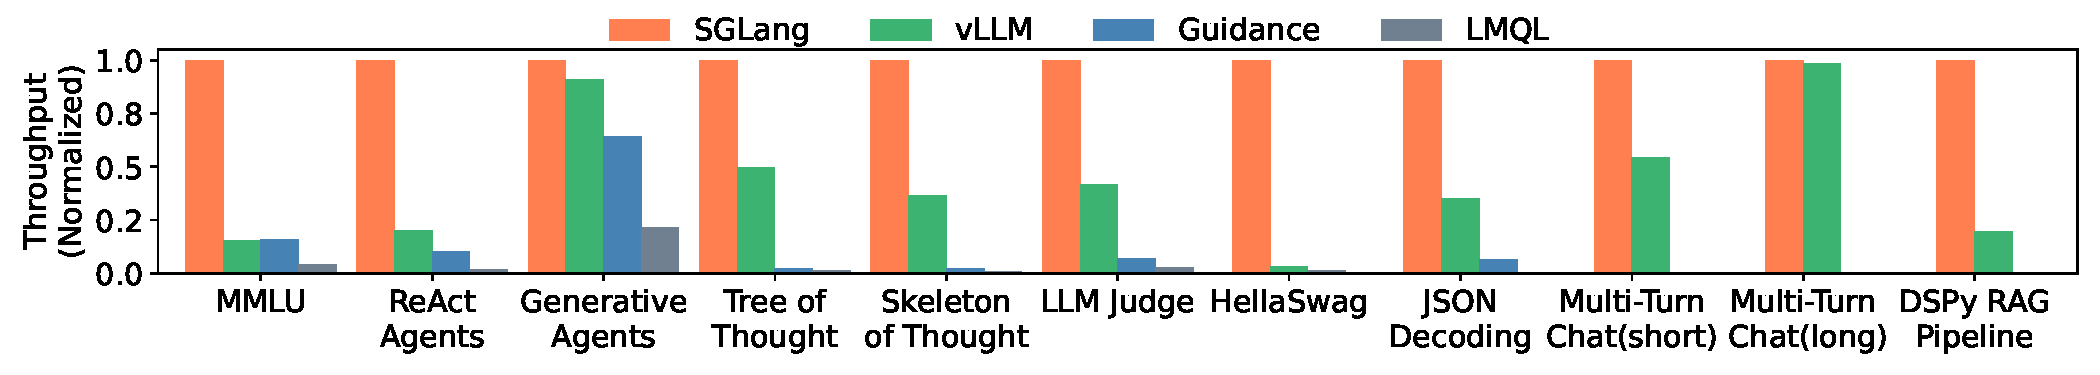
\includegraphics[width=\linewidth]{figures/e2e_throughput_llama_7b.pdf}
\vspace{-2.1em}
\caption{Normalized throughput on Llama-7B models. Higher is better.}
\vspace{-2em}
\label{fig:exp_llama_7b_throughput}
\end{figure}

\begin{figure}[t]
\centering
\vspace{-0.5em}
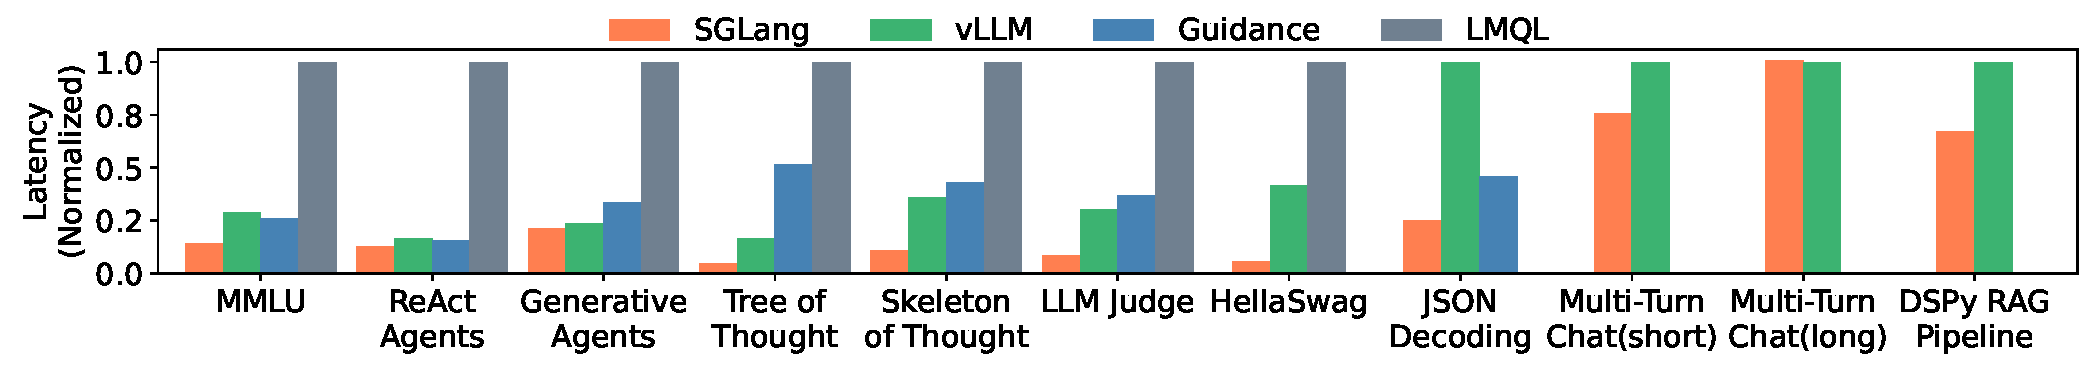
\includegraphics[width=\linewidth]{figures/e2e_latency_llama_7b.pdf}
\vspace{-2.1em}
\caption{Normalized latency on Llama-7B models. Lower is better.}
\vspace{-0em}
\label{fig:exp_llama_7b_latency}
\end{figure}

\subsection{End-to-End Performance}
\textbf{Results on open-weight models.} The latency and throughput results are shown in \autoref{fig:exp_llama_7b_throughput} and \autoref{fig:exp_llama_7b_latency}. \lang improves throughput by up to $6.4\times$ and reduces latency by up to $3.7\times$.
These improvements result from KV cache reuse, the exploitation of parallelism within a single program, and faster constrained decoding. Next, we explain the reasons for the speedup in each benchmark.

On MMLU, \lang can reuse the KV cache of the 5-shot examples with RadixAttention. RadixAttention benefits both throughput and latency. RadixAttention reduces total memory usage by sharing the KV cache, allowing for a larger batch size to improve maximum throughput. RadixAttention also reduces the computation of prefill, thus decreasing the first token latency. On HellaSwag, \lang reuses the KV cache of both few-shot examples and the common question prefix for multiple choices, resulting in two-level sharing. 
For the ReAct and generative agents, \lang reuses the KV cache of the agent template and previous calls. On Tree-of-thought and Skeleton-of-thought, \lang parallelizes the generation calls within a single program and reuses the KV cache as much as possible. On JSON decoding, \lang accelerates decoding by decoding multiple tokens at once with a compressed finite state machine. In multi-turn chat, \lang reuses the KV cache of the chat history. The speedup is more noticeable for short outputs because KV cache reuse mostly helps reduce the prefix time. For long outputs, because there is not much sharing between different chat sessions and the decoding time dominates, there is almost no speedup.
In the DSPy RAG pipeline, \lang reuses the KV cache of the common context example.
On these benchmarks, the cache hit rate ranges from 50\% to 99\%. 
\autoref{fig:exp_cache_hit_rate} (Appendix) lists the achieved and optimal cache hit rates for all of them, showing that our cache-aware scheduling approaches 96\% of the optimal hit rate on average.


We exclude LMQL and Guidance from some of the last five benchmarks due to slow performance and missing functionalities. LMQL's issues stem from slow token-level processing and an unoptimized backend, while Guidance lacks batching and parallelism support.


\begin{figure}[t]
\centering
\vspace{-1em}
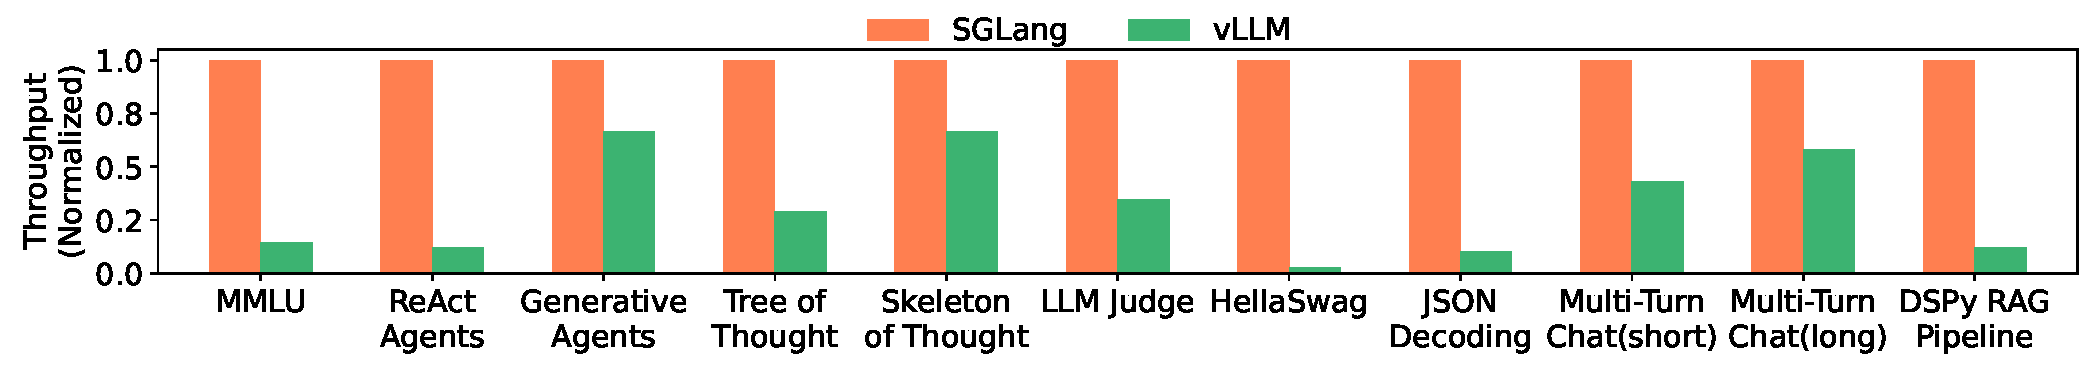
\includegraphics[width=\linewidth]{figures/e2e_throughput_mixtral_8x7b.pdf}
\vspace{-2.0em}
\caption{Normalized throughput on Mixtral-8x7B models with tensor parallelism. Higher is better.}
\vspace{-1.5em}
\label{fig:exp_mixtral_8x7b_throughput}
\end{figure}

\textbf{Results on larger models with tensor parallelism.}
We run larger models, Mixtral-8x7B and Llama-70B, with tensor parallelism on the same set of benchmarks and report the results in \autoref{fig:exp_mixtral_8x7b_throughput} and \autoref{fig:exp_llama_70b_throughput} (Appendix). The speedup on larger models shows a trend similar to that observed on smaller models, indicating that our optimization generalizes well to larger models.
We omit Guidance and LMQL here because they lack efficient implementations of tensor parallelism.

\textbf{Results on multi-modal models.}
\lang has native support for multi-modal models with the \texttt{image} and \texttt{video} primitives. The optimizations in this paper are compatible with multi-modal models. For RadixAttention, we compute the hash of the input images and use it as the key in the radix tree, allowing us to reuse the KV cache of the image tokens from the same image.
We run LLaVA-v1.5-7B (image) on llava-bench-in-the-wild and LLaVA-NeXT-34B (video) on ActivityNet. Because these models are not well supported by other baseline systems, we use the model authors' original implementation in Hugging Face Transformers as the baseline.
As shown in \autoref{tab:e2e_multi_modal}, \lang provides throughput up to $6\times$ higher on these benchmarks. In llava-bench-in-the-wild, there are multiple questions about the same image, and \lang runtime reuses the KV cache in this case.


\begin{table}[t]
\footnotesize
\centering
\vspace{-1.5em}
\caption{Throughput comparison on multi-modal LLaVA image and video models.}
\resizebox{0.8\columnwidth}{!}{
\begin{tabular}{ccc}
\toprule
Model                     & LLaVA-v1.5-7B (image) & LLaVA-NeXT-34B (video) \\
\midrule
Author's original implementation  &  0.18 image/s          &  0.02 frame/s            \\
\lang                     &  \textbf{1.15 image/s} & \textbf{0.10 frame/s}    \\
\bottomrule
\end{tabular}
}
\vspace{2em}
\label{tab:e2e_multi_modal}
\end{table}

\textbf{Production deployment.}
\lang has been deployed in Chatbot Arena~\cite{chiang2024chatbot} to serve open-weight models. Due to low traffic for some models, only one \lang worker serves each. After one month, we observed a 52.4\% RadixAttention cache hit rate for LLaVA-Next-34B~\cite{liu2024llavanext} and 74.1\% for Vicuna-33B~\cite{vicuna2023}. Cache hits come from common system messages, frequently reused example images, and multi-turn chat histories. This reduces first-token latency by an average of $1.7\times$ for Vicuna-33B.

\textbf{Results on API models.} We test a prompt that extracts three fields from a Wikipedia page using OpenAI's GPT-3.5 model. By using few-shot prompting, the accuracy of API speculative execution is high, and it reduces the cost of input tokens by about threefold due to the extraction of three fields.


\begin{figure}[t]
\centering
\vspace{-2.5em}
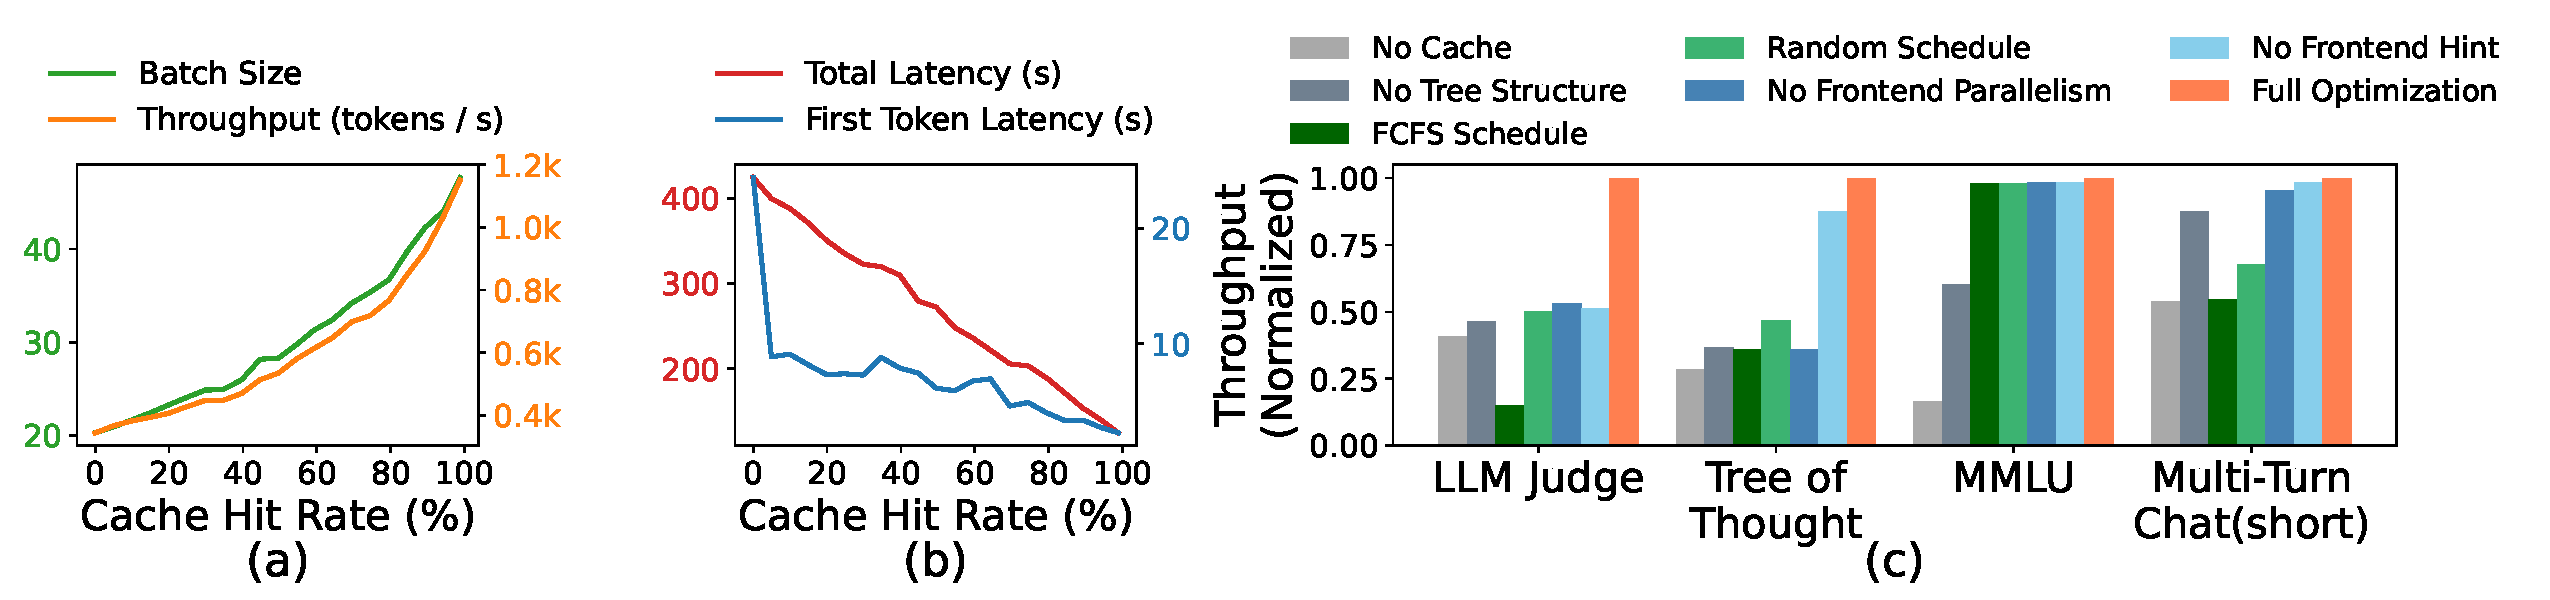
\includegraphics[width=\linewidth]{figures/cache_hit_and_ablation.pdf}
\vspace{-1.5em}
\caption{(a)(b) Cache hit rate ablation study. (c) RadixAttention ablation study.}
\vspace{-2em}
\label{fig:exp_hit_rate_vs_perf}
\end{figure}



\subsection{Ablation Study}

\textbf{Cache hit rate vs. latency/throughput.}
\autoref{fig:exp_hit_rate_vs_perf}(a)(b) shows the relationship between cache hit rate and performance metrics (first token latency, total latency, batch size, and throughput) on the tree-of-thought benchmark. The figure is obtained by partially disabling matched tokens at runtime. It shows that a higher cache hit rate leads to a larger batch size, higher throughput, and lower latency.

\textbf{Effectiveness of RadixAttention.}
We test the effectiveness of RadixAttention and its components on several representative benchmarks. As shown in \autoref{fig:exp_hit_rate_vs_perf}(c), "No Cache" means not using any cache, "No Tree-Structure" means using a simple table-based cache instead of a tree-structured cache, "FCFS Schedule" means using a first-come-first-serve policy instead of our cache-aware scheduling, "Random Schedule" means using a random order to schedule requests, "No Frontend Parallelism" means disabling parallelism in the interpreter, "No Frontend Hint" means disabling sending the fork hints from the interpreters, and "Full optimizations" means we turn on all optimizations. The experimental results show that each of these components is required to achieve the best performance. Disabling parallelism and hints from the frontend interpreter also results in suboptimal runtime performance, highlighting the importance of co-designing the frontend language and runtime.


\textbf{Overhead of RadixAttention.}
We test the overhead of RadixAttention on a benchmark without any KV cache reuse opportunities. The benchmark measures throughput on the ShareGPT dataset.
It takes 74.3 seconds to run 100 requests; however, the time used for managing the RadixAttention data structures is only 0.2 seconds, which is a negligible overhead of less than 0.3\%. This is because the complexity of tree operations is linear and small. Thus, we can turn on RadixAttention by default.

\textbf{Effectiveness of the compressed finite state machine.}
We test the effectiveness of the compressed finite state machine and its components on the JSON decoding benchmark.
Experimental results show that the compressed finite state machine increases the throughput by $1.6\times$ because it can decode multiple tokens at once. In addition, we need to preprocess the state machine and reuse it for a batch of requests. Otherwise, redoing the preprocessing for each request makes the throughput $2.4\times$ lower.












